%xelatex -shell-escape -output-directory=bin ergasia.tex
\documentclass{assignment}

\usepackage{enumerate} % Για την χρησιμοποίηση roman enumerate
\usepackage{pdflscape}
\usepackage{subcaption}


\university{Πανεπιστήμιο Πειραιώς}{Πα.Πει.}
\school{Τμήμα Πληροφορικής}{Π.Μ.Σ. "Πληροφορική"}
\department{Πρόγραμμα Μεταπτυχιακών Σπουδών «Πληροφορική»}{}
%\cover{images/cover.jpg}{http://www.cyberciti.biz/faq/grub-boot-into-single-user-mode/}

\title{Πιθανότητες και Στατιστική \\ Εργασία Εξαμήνου}
%\projectlevel{Εργαστήριο Λειτουργικά Συστήματα}
%\lesson{Λειτουργικά Συστήματα}{1}
\date{Αθήνα, 2014}

\author{Αναγνωστόπουλος Βασίλης - Θάνος}
%\register{ΜΠΠΛ13002}{1}

%\exercauthor{Αναγνωστόπουλος Βασίλης - Θάνος}{06107083}{9}

%\advisor{Τσακίρη Μαρία, Αναπληρώτρια Καθηγήτρια Ε.Μ.Π.}

\begin{document}

\maketitle
% Να σκεφτώ τί αλλαγές θέλω να κάνω με τις αριθμήσεις και άμα θέλω να κάνω.
% Να σκεφτώ να τις ενσωματώσω και στο assignment.cls

\setcounter{page}{1} 
\pagenumbering{roman}

\pagestyle{plain}
\tableofcontents
\newpage


%\pagestyle{headings}
\pagestyle{fancy}
\setcounter{page}{1} 
\pagenumbering{arabic}

\section{Εισαγωγή - Αντικείμενο της άσκησης}

Τα δεδομένα στο αρχείο \en{views.sav} αποτελούν τυχαίο δείγμα 52 σελίδων και περιέχουν τις ακόλουθες μεταβλητές:

\begin{table}[h]
\begin{center}
  \begin{tabular}{|m{0.30\textwidth}|m{0.50\textwidth}|}
    \hline
    {\bf Όνομα μεταβλητής} & {\bf Περιγραφή μεταβλητής} \\ \hline
    \en{Country}           & Χώρα προέλευσης (1 = ελληνική, 0 = όχι ελληνική) \\ \hline
    \en{Subject}           & Θεματολογία της ιστοσελίδας (1 = Αθλητικά, 2 = Πολιτικά, 3 = \en{Lifestyle}) \\ \hline
    \en{News}              & Ημερήσιος αριθμός νέων αναρτήσεων \\ \hline
    \en{Yr}                & Παλαιότητα της ιστοσελίδας (1 = λειτουργεί λιγότερο από 2 έτη, 0 = διαφορετικά) \\ \hline
    \en{Journalists}       & Αριθμός δημοσιογράφων που απασχολούνται στη συγκεκριμένη ιστοσελίδα \\ \hline
    \en{Views}             & Ετήσιος αριθμός επισκέψεων (\en{views}) σε συγκεκριμένη ιστοσελίδα \\ \hline
  \end{tabular}
\caption{Οι μεταβλητές του αρχείου \en{views.sav}.}
\label{table:variables}
\end{center}
\end{table}

Από το αρχικό αρχείο αφαιρέθηκε η 2 παρατήρηση με τιμές (0,1,12,1,22,35350)


\begin{Assignment}[Μέρος Α]
\AssignmentTitle{% 

\begin{itemize}
  \item Να υπολογισθεί ή μέση τιμή και η τυπική απόκλιση των ετήσιων αριθμών επισκέψεων των ιστοσελίδων. Να δοθεί η ερμηνεία των αποτελεσμάτων.
\end{itemize}
}

Μέσος όρος ή αλλιώς δειγματική μέση τιμή ενός συνόλου ν παρατηρήσεων είναι ένα μέτρο θέσης, δηλαδή δείχνει σχετικά τις θέσεις των αριθμών στους οποίους αναφέρεται. Γενικά, ορίζεται ως το άθροισμα των παρατηρήσεων δια του πλήθους αυτών. Είναι δηλαδή η μαθηματική πράξη ανεύρεσης της «μέσης απόστασης» ανάμεσα σε δύο ή περισσότερους αριθμούς. Η μέση τιμή συμβολίζεται με $\bar{x}$. Γενικός τύπος της μέσης τιμής είναι \cite{wiki:mean_value}:

\begin{equation}
\bar{x} = \frac{1}{n}\sum_{i=1}^n t_i = \frac{1}{n} (t_1+\cdots+t_n) 
\end{equation}

όπου $t_i$ η $i$ παρατήρηση και $n$ το πλήθος των παρατηρήσεων


Η διακύμανση ή διασπορά μίας τυχαίας μεταβλητής $x$ συμβολίζεται συνήθως με $Var[x]$ και δηλώνει πόσο συγκεντρωμένες γύρω από τη μέση τιμή είναι οι τιμές της τυχαίας μεταβλητής. Η θετική τετραγωνική ρίζα της διακύμανσης ονομάζεται τυπική απόκλιση και συμβολίζεται με $\sigma$. Ο γενικός τύπος της απόκλισης είναι \cite{wiki:variance}:

\begin{equation}
\sigma=\sqrt{\frac1{n-1}\sum_{i=1}^n(t_i-\bar{x})^2}
\end{equation}

Για τον υπολογισμό τους στο SPSS πηγαίνουμε στο μενού: \en{Analyze/Descriptive Statistics/Descriptives} (βλ. σχήμα \ref{fig:mean}) και προκύπτει ο πίνακας \ref{table:mean}.

\begin{table}[h]
\begin{center}
  \begin{tabular}{|c|c|c|c|}
    \hline
               &   N  & \en{Mean} & \en{Std. Deviation} \\ \hline 
    \en{views} & 51   & 23571.14  & 5743.964 \\ \hline
    \en{Valid N (listwise)} &51 & & \\ \hline
  \end{tabular}
\caption{Η μέση τιμή και η τυπική απόκλιση των ετήσιων αριθμών επισκέψεων των ιστοσελίδων.}
\label{table:mean}
\end{center}
\end{table}

\begin{figure}
  \centering
  \begin{subfigure}[b]{0.4\textwidth}
     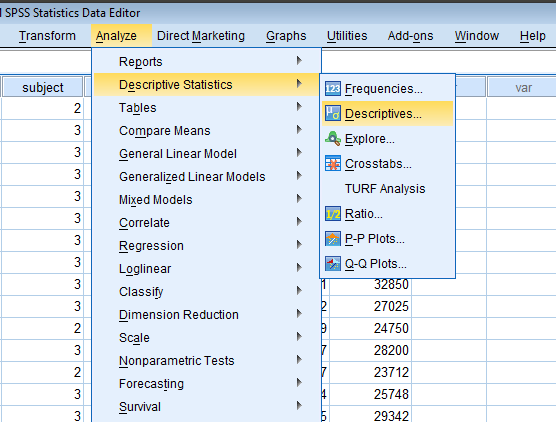
\includegraphics[width=\textwidth,height=0.15\textheight]{images/menu_mean.png}
     %\caption{A gull}
     %\label{fig:gull}
  \end{subfigure}%
   ~ %add desired spacing between images, e. g. ~, \quad, \qquad, \hfill etc.
          %(or a blank line to force the subfigure onto a new line)
  \begin{subfigure}[b]{0.4\textwidth}
    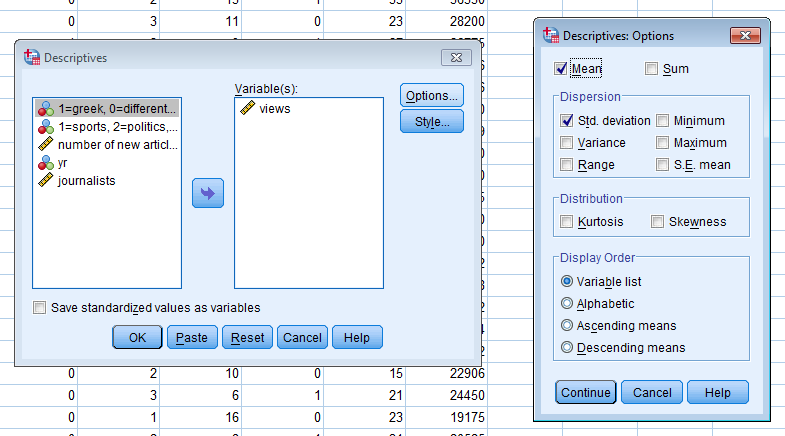
\includegraphics[width=\textwidth,height=0.15\textheight]{images/mean.png}
    %\caption{A tiger}
    %\label{fig:tiger}
  \end{subfigure}
  \caption{Το μενού Analyze/Descriptive Statistics/Descriptives του SPSS}
\label{fig:mean}
\end{figure}

Παρατηρούμε ότι η μέση τιμή είναι ίση με $23571,14$. Αυτό πρακτικά σημαίνει ότι η κεντρική τάση των επισκέψεων των ιστοσελίδων είναι $23571,14$. Πρόσθετα η τυπική απόκλιση του δείγματος των 51 δειγμάτων ισούται με $5743.964$. Η τυπική απόκλιση εκφράζει το βαθμό διασποράς των επισκέψεων των ιστοσελίδων, δηλαδή περιγράφει το αν το δείγμα των βαθμολογίων αποτελείται από παρατηρήσεις που έχουν κοντινές ή μακρινές αποστάσεις μεταξύ τους \cite{class_notes}.

\AssignmentTitle{% 

\begin{itemize}
  \item Να υπολογισθεί η διάμεσος, τα τεταρτημόρια, το 40\% ποσοστημόριο και η κορυφή των ετησίων αριθμών επισκέψεων των ιστοσελίδων. Να δοθεί η ερμηνεία των αποτελεσμάτων.
\end{itemize}

}

Διάμεσος ενός συνόλου ν παρατηρήσεων είναι η αριθμητική τιμή που διαχωρίζει το υψηλότερο ήμισυ ενός δείγματος δεδομένων, έναν πληθυσμό ή μία κατανομή πιθανοτήτων από το κάτω μισό \cite{wiki:median}.

Τεταρτημόριο είναι ένα μέτρο που χρησιμοποιείται στην στατιστική και υποδηλώνει την τιμή κάτω από την οποία ένα δεδομένο ποσοστό παρατηρήσεων βρίσκονται κάτω από αυτή την τιμή \cite{wiki:percentile}.

Κορυφή είναι η τιμή που εμφανίζεται πιο συχνά σε ένα σύνολο δεδομένων \cite{wiki:mode}.

Για τον υπολογισμό τους στο SPSS πηγαίνουμε στο μενού: \en{Analyze/Descriptive Statistics/Frequencies} (βλ. σχήμα \ref{fig:frequencies}) και προκύπτει ο πίνακας \ref{table:frequencies}.


\begin{table}[h]
\begin{center}
  \begin{tabular}{|c c|c|}
    \hline
    N                & \en{Valid}   & 51       \\ \hline
                     & \en{Missing} & 0        \\ \hline
    \en{Median}      &              & 23713.00 \\ \hline 
    \en{Mode}        &              & 28200    \\ \hline
    \en{Percentiles} & 25           & 18075.00 \\ \hline
    \en{Percentiles} & 40           & 21479.80 \\ \hline
    \en{Percentiles} & 50           & 23713.00 \\ \hline
    \en{Percentiles} & 75           & 27025.00 \\ \hline
  \end{tabular}
\caption{Η διάμεσος, τα τεταρτημόρια, το ποσοστημόριο και η κορυφή των ετήσιων αριθμών επισκέψεων των ιστοσελίδων.}
\label{table:frequencies}
\end{center}
\end{table}

Παρατηρούμε ότι η διάμεσος (\en{median}) είναι ίση με $23713$, που σημαίνει ότι οι 25 ιστοσελίδες έχουν μέχρι $23713$ επισκέψεις ενώ οι υπόλοιπες παραπάνω. Η κορυφή των παρατηρήσεων είναι $28200$, που σημαίνει ότι είναι η πιο συχνά εμφανιζόμενη τιμή. Τέλος το πρώτο τεταρτημόριο είναι ίσο με $18075$ (που σημαίνει ότι το 1/4 των ιστοσελίδων έχουν επισκέψεις μέχρι $18075$) και ομοίως και για τα υπόλοιπα. Το ποσοστημόριο 40\% ισούται με $21479.80$ που ομοίως σημαίνει ότι το 30\% των σελίδων έχουν επισκέψεις μέχρι και $21479.80$ .

\begin{figure}
  \centering
  \begin{subfigure}[b]{0.4\textwidth}
     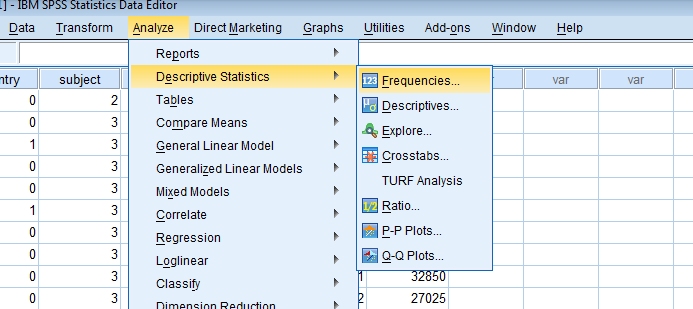
\includegraphics[width=\textwidth,height=0.15\textheight]{images/menu_frequencies.png}
  \end{subfigure}%
   ~ %add desired spacing between images, e. g. ~, \quad, \qquad, \hfill etc.
  \begin{subfigure}[b]{0.4\textwidth}
    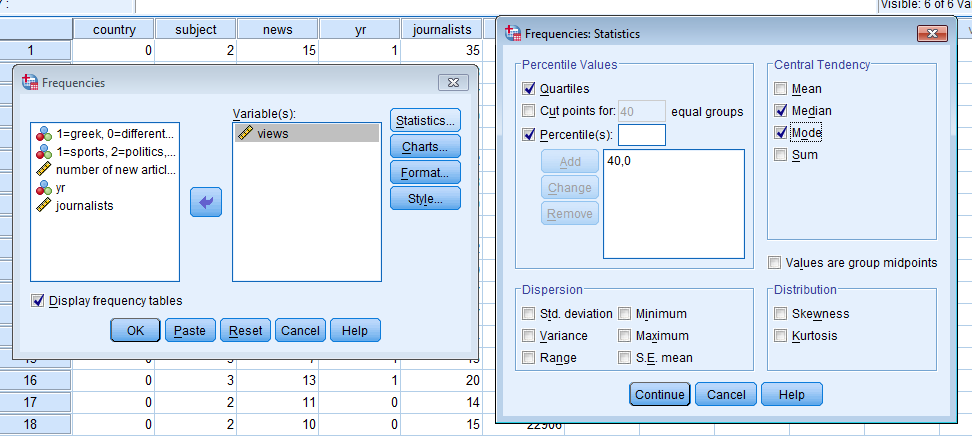
\includegraphics[width=\textwidth,height=0.15\textheight]{images/frequencies.png}
  \end{subfigure}
  \caption{Το μενού Analyze/Descriptive Statistics/Frequencies του SPSS}
\label{fig:frequencies}
\end{figure}

\AssignmentTitle{% 

\begin{itemize}
  \item Να ορισθεί κατάλληλα μια νέα μεταβλητή (\en{Views\_2}), η οποία να ομαδοποιεί τις ιστοσελίδες σε 4 κατηγόριες ανάλογα με τον ετήσιο αριθμό επισκέψεων τους ως εξής:
  \begin{description}
    \item [1\textsuperscript{η} ομάδα:] ιστοσελίδες με ετήσιο αριθμό επισκέψεων μέχρι 22000
    \item [2\textsuperscript{η} ομάδα:] ιστοσελίδες με ετήσιο αριθμό επισκέψεων πάνω από 22000 και μέχρι 28000
    \item [3\textsuperscript{η} ομάδα:] ιστοσελίδες με ετήσιο αριθμό επισκέψεων πάνω από 28000 και μέχρι 30000
    \item [4\textsuperscript{η} ομάδα:] ιστοσελίδες με ετήσιο αριθμό επισκέψεων πάνω από 30000 
  \end{description}
  \begin{itemize}
    \item Να κατασκευασθεί ο πίνακας συχνοτήτων και το κυκλικό διάγραμμα βάσει της νέας μεταβλητής
    \item Τί ποσοστό των ιστοσελίδων ανήκουν στην 3\textsuperscript{η} ομάδα;
  \end{itemize}
\end{itemize}

}

Για τον υπολογισμό τους στο SPSS πηγαίνουμε στο μενού: \en{Analyze/Descriptive Statistics/Frequencies} και προκύπτει ο πίνακας \ref{table:frequencies:Views_2}.

\begin{table}[h]
\begin{center}
  \begin{tabular}{|c c|c|c|c|c|c|}
    \hline
       & & \en{Frequency}  & \en{Percent}  & \en{Valid Percent}  & \en{Cumulative Percent} \\ \hline
    \en{Valid}  &  1.00        &  21  &  41.2  &  41.2  &  41.2  \\ \hline 
                &  2.00        &  19  &  37.3  &  37.3  &  78.4  \\ \hline
                &  3.00        &  4   &  7.8   &  7.8   &  86.3  \\ \hline
                &  4.00        &  7   &  13.7  &  13.7  &  100.0 \\ \hline
                &  \en{Total}  &  51  &  100.0 &  100.0 &        \\ \hline
  \end{tabular}
\caption{Ο πίνακας συχνοτήτων της μεταβλητής \en{Views\_2}.}
\label{table:frequencies:Views_2}
\end{center}
\end{table}

\begin{figure}
  \centering
  \resizebox*{16.5cm}{!}{
    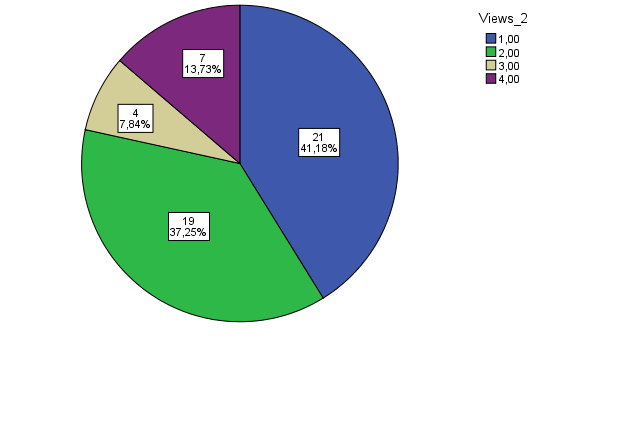
\includegraphics{images/views_2_pie.png}
  }
  \caption{Το μενού Analyze/Descriptive Statistics/Frequencies του SPSS}
\label{fig:frequencies}
\end{figure}


\AssignmentTitle{% 
\begin{itemize}
  \item Να συγκριθούν ως προς τη μεταβλητότητα που παρουσιάζουν οι 4 ομάδες ιστοσελίδων που έχουν δημιουργηθεί βάσει της νέας μεταβλητής (\en{Views\_2}). Σχολιάστε τα αποτελέσματα.
\end{itemize}
}

\begin{table}[h]
\begin{center}
  \begin{tabular}{|c c|c|}
    \hline
    N                & \en{Valid}   & 51       \\ \hline
                     & \en{Missing} & 0        \\ \hline
    \en{Median}      &              & 2.000    \\ \hline 
    \en{Mode}        &              & 1.00     \\ \hline
    \en{std. Deviation}&            & 1.02785  \\ \hline
    \en{Variance}    &              & 1.056    \\ \hline
    \en{Range}       &              & 3.000    \\ \hline
    \en{Percentiles} & 25           & 1.00     \\ \hline
    \en{Percentiles} & 50           & 2.00     \\ \hline
    \en{Percentiles} & 75           & 3.00     \\ \hline
  \end{tabular}

\caption{Η διάμεσος, τα τεταρτημόρια, το ποσοστημόριο και η κορυφή των ετήσιων αριθμών επισκέψεων των ιστοσελίδων.}
\label{table:frequencies:views_2}
\end{center}
\end{table}

%http://en.wikipedia.org/wiki/Statistical_variability

\end{Assignment}

\begin{Assignment}[Μέρος Β]
\AssignmentTitle{ % 
\begin{itemize}
  \item Να εξετασθεί σε επίπεδο σημαντικότητας 5\% αν οι ελληνικές ιστοσελίδες έχουν την ίδια μέση ετήσια επισκεψιμότητα με τις όχι ελληνικές ιστοσελίδες.
\end{itemize}
}

\AssignmentTitle{ % 
\begin{itemize}
  \item Να εξετασθεί σε επίπεδο σημαντικότητας 5\% αν οι ιστοσελίδες που λειτουργούν τουλάχιστον 2 έτη, έχουν τον ίδιο μέσο ετήσιο αριθμό επισκέψεων με ιστοσελίδες που λειτουργούν λιγότερο από 2 έτη.
\end{itemize}
}

\AssignmentTitle{ % 
\begin{itemize}
  \item Να εξετασθεί σε επίπεδο σημαντικότητας 5\% αν ο μέσος ετήσιος αριθμός επισκέψεων των ιστοσελίδων είναι στατιστικά ίσος μς 25000 ή όχι.
\end{itemize}
}

\AssignmentTitle{ % 
\begin{itemize}
  \item Να εξετασθεί σε επίπεδο σημαντικότητας 5\% αν ο παράγοντας \en{Country} επηρεάζει τη θεματολογία της ιστοσελίδας.
\end{itemize}
}

\end{Assignment}

\begin{Assignment}[Μέρος Γ]
\AssignmentTitle{ % 
\begin{itemize}
  \item Να εξετασθεί αν η μεταβλητή \en{views} ($Y$) εξαρτάται γραμμικά από τις μεταβλητές, \en{country, subject, news, journalist, yr}. Να βρεθεί το βέλτιστο γραμμικό μοντέλο (σε επίπεδο σημαντικότητας 1\%) και να δοθεί η γραμμική εξίσωση που αντιστοιχεί σε αυτό.
ελληνικής με τα ίδια χαρακτηριστικά.
\end{itemize}
}

\AssignmentTitle{ % 
\begin{itemize}
  \item Χρησιμοποιώντας το πλήρες μοντέλο, να εκτιμηθούν οι συντελεστές της γραμμική του εξίσωσης. Να δοθεί η ερμηνεία των αποτελεσμάτων. 
\end{itemize}
}

\AssignmentTitle{ % 
\begin{itemize}
  \item Χρησιμοποιώντας το πλήρες μοντέλο, να εκτιμηθεί σημειακά και με διάστημα εμπιστοσύνης 99\% ο αναμενόμενος επιπρόσθετος ετήσιος αριθμός επισκέψεων, που θα παρουσιάσει μία ελληνική ιστοσελίδα, έναντι μίας όχι ελληνικής με τα ίδια χαρακτηριστικά.
\end{itemize}
}

\end{Assignment}

\begin{Assignment}[Μέρος Δ]
\AssignmentTitle{ % 
Δημιουργούμε μία νέα μεταβλητή (\en{journalists\_2}) που ομαδοποιεί τις ιστοσελίδες ανάλογα με τον αριθμό δημοσιογράφων που απασχολούν ως ακολούθως:
\begin{description}
  \item [1\textsuperscript{η} ομάδα:] ιστοσελίδες με αριθμό δημοσιογράφων μέχρι 8
  \item [2\textsuperscript{η} ομάδα:] ιστοσελίδες με αριθμό δημοσιογράφων πάνω από 8 μέχρι και 20
  \item [3\textsuperscript{η} ομάδα:] ιστοσελίδες με αριθμό δημοσιογράφων πάνω από 20
\end{description}
\begin{itemize}
  \item Εφαρμόζοντας κατάλληλο στατιστικό μοντέλο, να εξετασθεί σε επίπεδο σημαντικότητας 5\%, αν ο ετήσιος αριθμός επισκέψεων μίας ιστοσελίδας εξαρτάται από το αν η ιστοσελίδα ανήκει στην 1\textsuperscript{η}, 2\textsuperscript{η} ή 3\textsuperscript{η} ομάδα βάσει του παράγοντα \en{journalists\_2} και από τη χώρα προέλευσης. Δώστε την τελική μορφή του μοντέλου στην οποία καταλήξατε και σχολιάστε τα αποτελέσματα.
\end{itemize}
}

\AssignmentTitle{ % 
\begin{itemize}
  \item Χρησιμοποιώντας την τελική μορφή του μοντέλου που καταλήξατε στο ερώτημα (1), να δοθούν οι σημειακές εκτιμήσεις και τα διαστήματα εμπιστοσύνης 95\% για τους μέσους ετήσιους αριθμούς επισκέψεων των ιστοσελίδων για κάθε μία από τις ομάδες που έχουν σχηματισθεί βάσει της μεταβλητής \en{journalists\_2}. Σχολιάστε και τα αποτελέσματα.
\end{itemize}
}

\end{Assignment}

\begin{Assignment}[Μέρος Ε]
\AssignmentTitle{ % 
\begin{itemize}
  \item Να εφαρμοσθεί κατάλληλη στατιστική μέθοδος ώστε να διευκρινιστεί το αν οι μεταβλητές \en{journalists, country, subject, news} που αντιστοιχούν σε μία ιστοσελίδα είναι επαρκείς πληροφορίες ώστε να μπορούμε να προβλέψουμε την παλαιότητα της συγκεκριμένης ιστοσελίδας. Να βρεθεί το βέλτιστο μοντέλο πρόβλεψης σε επίπεδο σημαντικότητας 10\% και να δοθεί η εξίσωση που αντιστοιχεί σε αυτό.
\end{itemize}
}

\AssignmentTitle{ % 
\begin{itemize}
  \item Χρησιμοποιώντας το βέλτιστο μοντέλο, να προβλεφθεί η παλαιότητα μίας ελληνικής ιστοσελίδας για την οποία γνωρίζουμε ότι απασχολεί 12 δημοσιογράφους, πραγματεύεται θέματα αθλητικής επικαιρότητας και στην οποία αναρτώνται ημερησίως 15 νέα άρθρα.
\end{itemize}
}

\end{Assignment}


\phantomsection \label{Βιβλιογραφία}
\addcontentsline{toc}{section}{Βιβλιογραφία}
%\mtcaddchapter[Βιβλιογραφία] % Λόγω του minitoc
\bibliographystyle{plain}
\bibliography{references}

\newpage

\end{document}

